\documentclass[
	classe=$1^{ere}STI2D$
]{exercice}

\usepackage{tkz-tab}

\title{Activité : étude d'une fonction de degré 2}

\begin{document}

\maketitle

On considère la fonction $f(x) = -\frac{1}{2}x² + \frac{1}{2}x + 6$.

\begin{enumerate}
	\item Quel est le point $x$ où la fonction est maximale ? Quelle est alors la valeur de $f(x)$ ?

	      \correction{$x$ est maximale en $x = -\frac{b}{2a} = 0,5$. Ainsi $f(x) = 6,125$.}
	\item En déduire le tableau de variations de $f$ :
	      \begin{center}
		      \begin{tikzpicture}
			      \tkzTabInit{$x$ / 1 , $f(x)$ / 2}{$\correction{-∞}$, $\correction{0,5}$, $\correction{+∞}$}
			      \ifdefined\makeCorrection
				      \tkzTabVar{-/ $-∞$, +/ $6{,}125$, -/ $-∞$}
			      \fi
		      \end{tikzpicture}
	      \end{center}
	\item Tracer la courbe de $f$ dans le repère ci-dessous :

	      \begin{center}
		      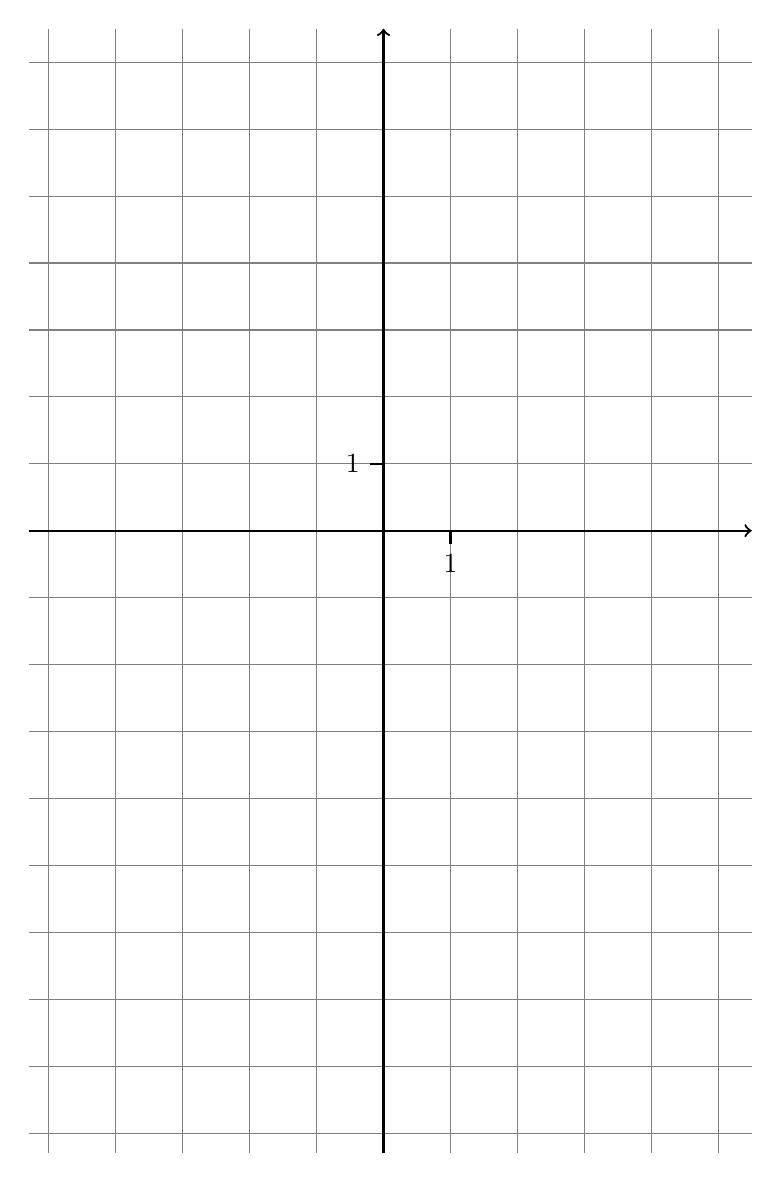
\begin{tikzpicture}[scale=0.85]
			      \newcommand{\AxeXDebut}{-5}
			      \newcommand{\AxeXFin}{5}
			      \newcommand{\AxeYDebut}{-9}
			      \newcommand{\AxeYFin}{7}
			      \draw[thin,gray] (\AxeXDebut-0.3,\AxeYDebut-0.3) grid (\AxeXFin+0.5,\AxeYFin+0.5);
			      \draw[thick,->] (\AxeXDebut-0.3,0) -- (\AxeXFin+0.5,0);
			      \draw[thick,->] (0,\AxeYDebut-0.3) -- (0,\AxeYFin+0.5);
			      \draw[thick] (1,0) -- ++(0,-0.2) node[below] {$1$};
			      \draw[thick] (0,1) -- ++(-0.2,0) node[left] {$1$};

			      \ifdefined\makeCorrection
				      \draw[red,variable=\x,domain=\AxeXDebut:\AxeXFin] plot({\x},{-0.5*(\x + 3)*(\x - 4)});
			      \fi
		      \end{tikzpicture}
	      \end{center}
	\item Déterminer graphiquement les racines $r₁$ et $r₂$ de $f$

	      $r₁ = \correctionDots{-3}$\hspace{2em} $r₂ = \correctionDots{\phantom{-}4}$
	\item Montrer que $f(x) = -\frac{1}{2}(x - r₁)(x - r₂)$.
\end{enumerate}

\end{document}